%%%%%%%%%%%%%%%%%%%%%%%%%%%%%% -*- Mode: Latex -*- %%%%%%%%%%%%%%%%%%%%%%%%%%%%
%% project-plan.tex -- 
%% Author          : Philip Johnson
%% Created On      : Tue Mar 31 11:44:58 2009
%% Last Modified By: Philip Johnson
%% Last Modified On: Wed Dec 16 15:29:18 2009
%% RCS: $Id$
%%%%%%%%%%%%%%%%%%%%%%%%%%%%%%%%%%%%%%%%%%%%%%%%%%%%%%%%%%%%%%%%%%%%%%%%%%%%%%%
%%   Copyright (C) 2009 
%%%%%%%%%%%%%%%%%%%%%%%%%%%%%%%%%%%%%%%%%%%%%%%%%%%%%%%%%%%%%%%%%%%%%%%%%%%%%%%
%% 

\section{Research plan}

% {\em The proposed research must approach fundamental research from an interdisciplinary perspective that integrates computing and communications with domain sciences and engineering to address the sustainability issues of interest. The proposal must describe a synergistic approach by which the team addresses scientific challenges in sustainability.}

Our research plan builds upon our 2014 pilot study with three phases: {\em Design and implementation}, {\em Deployment}, and {\em Assessment}.  The design and implementation phase will last approximately six months and will complete the second generation hardware and software systems now under development. The deployment phase will follow the design and implementation phase and last approximately one year. Deployment involves the distribution of our hardware to three neighborhoods and collection of power quality data.  The assessment phase will begin in parallel with deployment and last one and a half years. 

\subsection{2014 Pilot Study}

We performed a two month pilot study in August 2014 using our first generation OPQBox hardware and OPQHub software \cite{g1-pilot-study}. The pilot study involved the installation of three OPQBoxes in a scientific laboratory building on the UH Manoa campus, an apartment complex in Honolulu, and a residence on the Windward side of Oahu. These devices generated over 8000 voltage events (i.e. voltages outside the range of 114 - 126 V, exceeding the 5\% variability for normal operation established by our utility).  The devices also generated 16 frequency events (i.e. frequency fluctuation outside the range of 59.5 - 60.5 Hz). Our first generation OPQHub serverimplements a simple analytic to classify events according to the ITIC/CBEMA power tolerance curve \cite{ITIC}. During the pilot study period, our devices detected two abnormal power quality events according to this metric. We were also able to distinguish between local and grid-level power quality events, and even correlate power quality fluctuations to PV output.

This pilot study validated our hypothesis that our approach could provide useful information about the grid. It also produced valuable findings about the shortcomings of our first generation hardware and software.  For this project, we will build upon these preliminary findings with improved hardware, software and analytics. 

\subsection{Phase 1: Design and implementation}

\subsubsection{OPQ Hardware Device}

\begin{wrapfigure}{r}{4in}
  \includegraphics[width=0.6\textwidth]{figures/opq2.eps}
  \caption{\em \small Hardware block diagram}
  \label{fig:hardware-block-diagram}
\end{wrapfigure} 

Figure \ref{fig:hardware-block-diagram} shows a block diagram of our second generation OPQBox hardware device \cite{opqbox2}. It can be plugged into a standard U.S. two prong outlet with expected power at a frequency of 60 Hz and with a voltage of 120 V. It can operate under a frequency range of 50 Hz to 70 Hz and under a voltage range of 80 Vac to 200 Vac. Sampling is phase locked to the utility frequency. The 16 bit 100KSPS ADC allows for 5mV resolution with over 1024 points per grid cycle. On board ARM floating point DSP is able to perform the IEEE 1159 outlined analysis, as well as user defined code. 

OPQBox also includes 512k of ferromagnetic RAM (FRAM). FRAM will be used as a circular buffer, containing up to 1 min of high resolution voltage measurements. FRAM will maintain its state through a power cycle, which will be sent to the OPQHub once the OPQBox comes back online.

OPQBox is meant to bypass power filters and surge protectors. Thus, it incorporates extra protection elements to keep the device operating safely during power disruptions. Fuses will disable OPQBox2 in case of a fault. All of the user accessible components are isolated from the mains.

Finally, this generation OPQBox uses a Raspberry PI for WiFi-based communication with the OPQHub. (Future generations will use custom components to reduce size and cost.)

\subsubsection{OPQ Cloud-based software service}

In parallel with hardware, we have developed a cloud-based service for collection and analysis of the data. All source code is licensed under the GPL V3 and is available on GitHub \cite{opq-github}.  When a consumer receives a device, they use a browser to access our service and register their device. This includes specifying the kinds of alerts desired and how o receive them (email or text message).  Users can specify both thresholds for event triggering, frequency of alert delivery (immediately, or as part of a daily or weekly summary), and whether they want to be alerted to only their own quality events or to quality events (and annotations of these events) in their neighborhood.  

Device registration also includes a privacy-preserving means to specify the location of the hardware device. This is accomplished by presenting users with a map overlaid with zoomable tiles allowing them to select the device location with resolutions from 500 square feet (typically revealing the actual building containing the device) to 1 square mile (revealing only the neighborhood containing the device). This is illustrated in Figure \ref{fig:cloud-grid}.

\begin{wrapfigure}{r}{3.25in}
  \includegraphics[width=0.5\textwidth]{figures/cloud-grid.eps}
  \caption{\em \small Cloud service page illustrating zoomable grid}
  \label{fig:cloud-grid}
\end{wrapfigure}  


There are two additional forms of energy data that the user can allow OPQ to collect.  Some users may have PV and/or smart meters installed that provide internet access to consumption and/or generation data.  When available (and if the user is willing to share this data), OPQ can potentially have access to consumption, generation, and quality data about a single household.

After registration, OPQHub sends events to the user as specified during registration.  Beyond simple numerical data, the service can provide interpretation of the data, such as whether the frequency and/or severity of events is relatively low or high, and if high, actions that the user might want to consider.  These actions could include: (1) contacting the utility to request service (contact information supplied in the email); (2) Communicating with neighbors to see if they have power quality problems (via the creation of public annotations of their events); or (3) advice regarding actions (such as installation of UPS line conditioning for sensitive electronics, or unplugging them during events such as thunderstorms) depending upon the frequency/severity of power quality problems.

\subsection{Phase 2: Deployment}

After the hardware is designed and a small pilot manufacturing run has established device quality, we will manufacture 150 units for trial deployment.  Although our current hardware design requires WiFi, the 2012 US Census Report indicates that 85\% of Hawaii households have internet access \cite{home-internet-access}, so we do not expect this to be a problematic constraint. 

Our deployment will begin by dividing the units among three Oahu neighborhoods based upon the penetration of photovoltaics on their associated circuit.  Our utility publishes a ``Locational Value Map'' indicating the penetration of PV on a daily basis \cite{lvm}, and we will use this to choose one neighborhood with low penetration (i.e. where PV comprises less than 50\% of the circuit's daytime minimum load), medium penetration (i.e. where PV comprises 75\% to 100\% of the circuit's daytime minimum load) and high penetration (i.e. where PV comprises 120\% or greater of the circuit's daytime minimum load). 

Within a single neighborhood, we will choose participants to receive devices in order to obtain households both with and without photovoltaics. We want to obtain variety in monthly electricity bills (small being below \$50, medium being between \$50 and \$150, and large being above \$150).  We hope at least 20\% of the households will opt-in to providing consumption and/or generation data in addition to power quality data. 

To facilitate deployment, we will request the aid of local environmental and sustainablity groups.  Hardware devices will be provided free of charge to participants, with their incentive for participation being increased access to information about their household power quality.  

Our devices will be installed with a unique ID that is sent with each communication to the cloud-based service to identify the originating device.  We can use this information to determine whether users have installed and configured the device successfully, and if a previously functioning device has ceased to transmit data.   In either of these cases, we will contact the user to see if they no longer wish to participate and if so, retrieve the device for redistribution. 

We plan to collect data during the Deployment phase for at least six months. However, if the deployment is proceeding successfully we will continue with data collection for up to 18 months (or the end of the grant period).  Further data collection at that point will depend upon the availability of funds for the cloud-based service.

During the course of deployment we will be accessing online NOAA weather data to collect environmental data (temperature, humidity, winds, insolation) for the neighborhoods selected for participation. 

In parallel with the deployment phase, we will begin the Assessment phase. 

\subsection{Phase 3: Assessment}

Assessment of this project will involve both qualitative (questionnaire) and quantitative (power quality) data, and is designed to provide insight into the general research questions presented in Section \ref{sec:vision} as well as test several specific hypotheses described below. Our assessment procedure is as follows:

First, we will ask users to fill out a questionnaire when they receive their hardware device.  The questionnaire will assess their attitudes toward the electrical utility and the Smart Grid as well as their current electricity-related behaviors (i.e. recent electric bill amount indicating their consumption, presence of PV installation, use of hybrid or electric car). This will provide baseline information regarding attitude and behavior that we can use to assess the impact of access to power quality data.

Second, we will monitor the data over the course of deployment in order to ensure that hardware devices are being used, that they maintain high levels of uptime, and that power quality alerts are being observed and sent to users.  Based upon our experience with household installation of an AC Scout, we are confident that power quality problems will be observed in a significant fraction of the households.  In the event that a deployment does not generate a significant number of alerts in a given neighborhood after three months, we will manufacture additional devices and deploy to additional neighborhoods as necessary until we are able to obtain enough alerts to test our hypotheses.

Third, as soon as deployment begins, we will begin analysis of the collected power quality data to see if we can determine relationships with the environmental data we are also collecting. 

Fourth, upon conclusion of the deployment phase, we will ask users to fill out a second questionnaire.  This questionnaire will ask many of the same questions as the initial questionnaire, but will also ask if users made any changes with respect to their electrical behavior during the study period (such as installation of PV, installation of line conditioners, buying a hybrid vehicle, etc.) and to what extent these changes were motivated by information about their power quality.  This pre and post-test design will provide evidence regarding the ability of power quality data to enable active participation in the Smart Grid.  In addition to this self-reported data, we will also be able to observe ``active participation'' in the form of annotations users provide to their timeline.

Based upon analysis of the qualitative and quantitative data, we will test the following specific hypotheses: (1) Knowledge of personal power quality problems leads to actions such as contacting the utilities, installing UPS, or unplugging on alerts; (2) Intrinsic motivators (insight into personal and neighborhood power quality) plus a free device will suffice for participation in crowdsourced data collection; (3) Knowledge of neighborhood power quality issues leads to active engagement with neighbors; (4) Consumers find the recommendations provided by the OPQ system to be useful; (5) The frequency and severity of events is positively correlated with the degree of penetration of distributed PV on that circuit; (6) Consumers find crowdsourced power quality data to be more useful than their own power quality in isolation; (7) Participation is positively correlated with high monthly bills, installation of rooftop PV, or high numbers of severe PQ events.
















